\chapter{Design Description}

\section{Overview}
A Gain/Phase Analyzer is an instrument used to plot the frequency response of a
network or amplifier. The project, sponsored by Professor Kyle Temkin,
specifies a small, computer controlled gain/phase analyzer for use by students
and individuals. It can stimulate and then measure filters, amplifiers and
control systems, allowing their behavior to be plotted and analyzed. The device
is to be developed as an open-source project, so that students may study its
inner workings.

\section{Detailed Description}
Our project lacks many various and viable implementation
possibilities. As such, many major decisions will involve study of other
instrumentation which performs similar tasks, including a few open-source
network analyzers. Trade study will be used as required for selecting high-cost
components or designs of subsystems, and this will be addressed as necessary
during the development cycle. Hardware is being designed and  implemented in
different stages in order to ease the process of design. Software will be
created with the purpose of interfacing with the microcontroller.

\subsection{Synthesizer}
The first subsystem that will be built is the frequency synthesizer. This needs
to generate a frequency up to $150\;\mr{MHz}$. For this design, the circuit uses
the AD9958 Direct Digital Synthesis (DDS) chip and a `video' op-amp to produce
the correct output.

\begin{figure}[H]
\centering
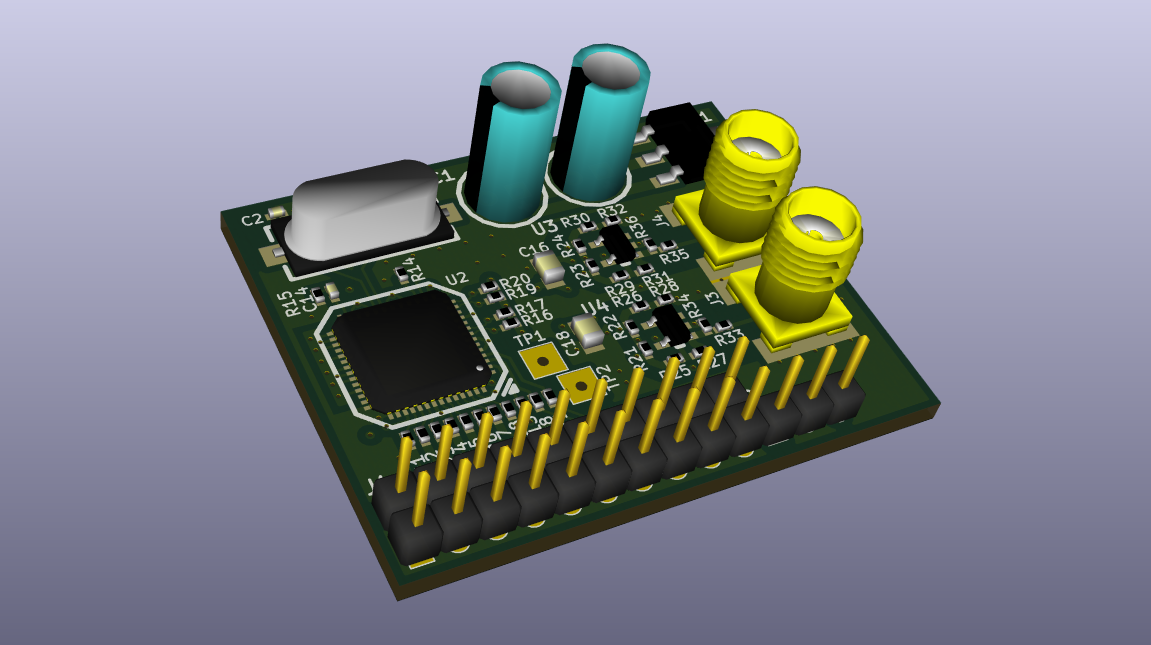
\includegraphics[width=4in]{synth3d.png}
\caption{Synthesizer PCB, 3D render}
\label{fig:synth3d}
\end{figure}

In the final product, we may integrate an optional CPLD or FPGA to allow the user
to drive the modulation feature of the DDS chip; for the purposes of testing we
have tied the modulation inputs straight to ground, as we do not require them.

\subsection{Input Front-end}
The next section of the design is the input front-end subsystem.

\begin{figure}[H]
\centering
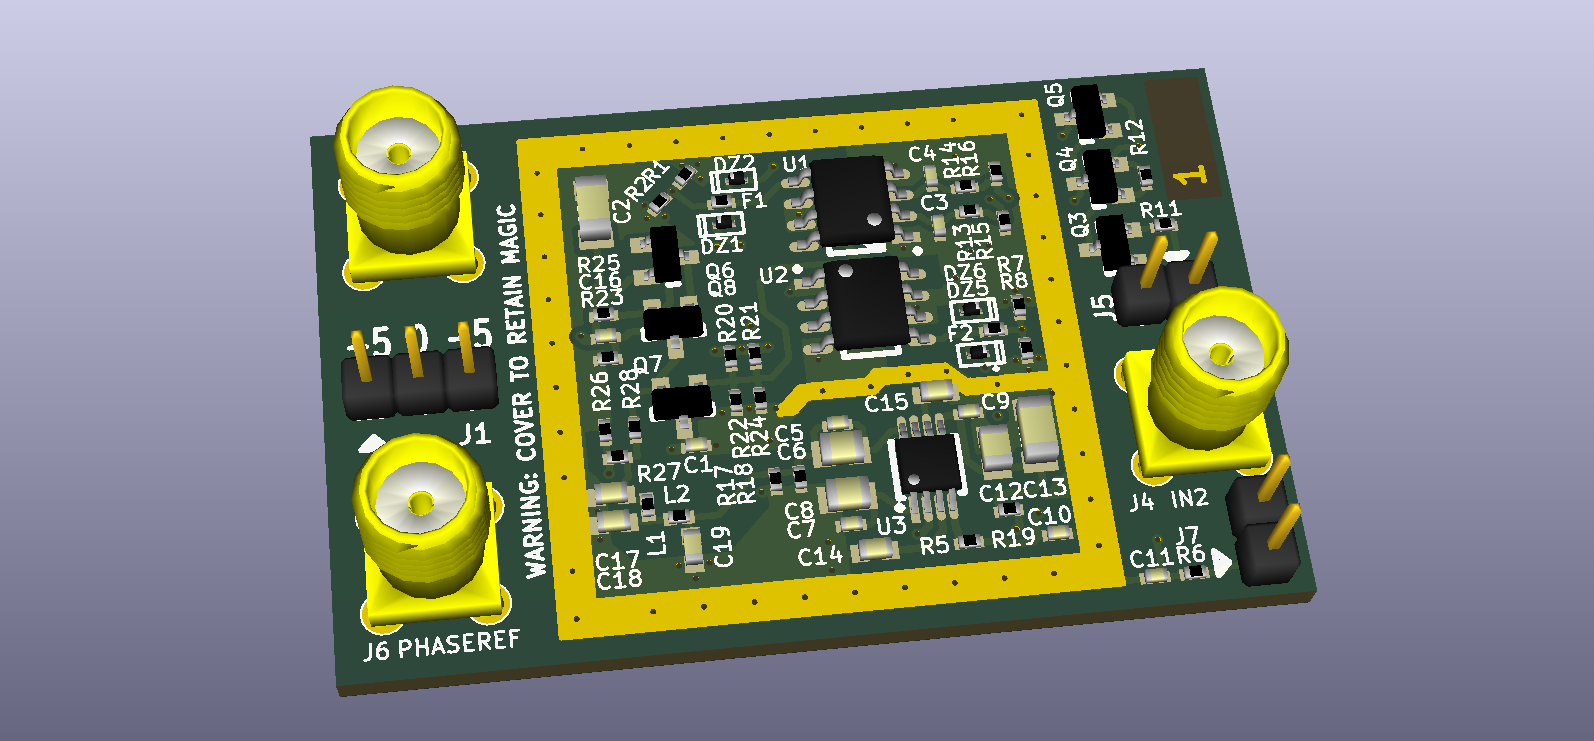
\includegraphics[width=4in]{frontend3d.png}
\caption{Input Front-end PCB, 3D render}
\label{fig:front3d}
\end{figure}

Our input front-end must take the signals from the front-panel input connectors
and present them in a form which can be directly sampled by the
microcontroller's analog-to-digital converter. The signals first pass through a
simple input protection circuit. This consists of a small-footprint SMD fuse in
series with the input and a clamping arrangement set around $3.3\;\mr{V}$
($23\;\mr{dBm}$ peak).  After the input protection, the two input signals enter
a switching circuit to select between them. This allows all of the following
circuitry to be shared between channels, minimizing cost and inter-channel
variation. This is followed by a buffer, which isolates the input signal from
the following power combiner and filter. After that, a power combiner adds in a
variable phase reference, which allows the system to measure the input signal's
phase, and a filter cuts the signal off at $300\;\mr{MHz}$. The filtered signal
then passes into a logarithmic detector with integrated low-pass filter, which
presents a voltage proportional to the logarithm of the input amplitude to the
microcontroller.

\subsection{Output Amplifier}
The next section of the design is the output amplifier subsystem.

\begin{figure}[H]
\centering
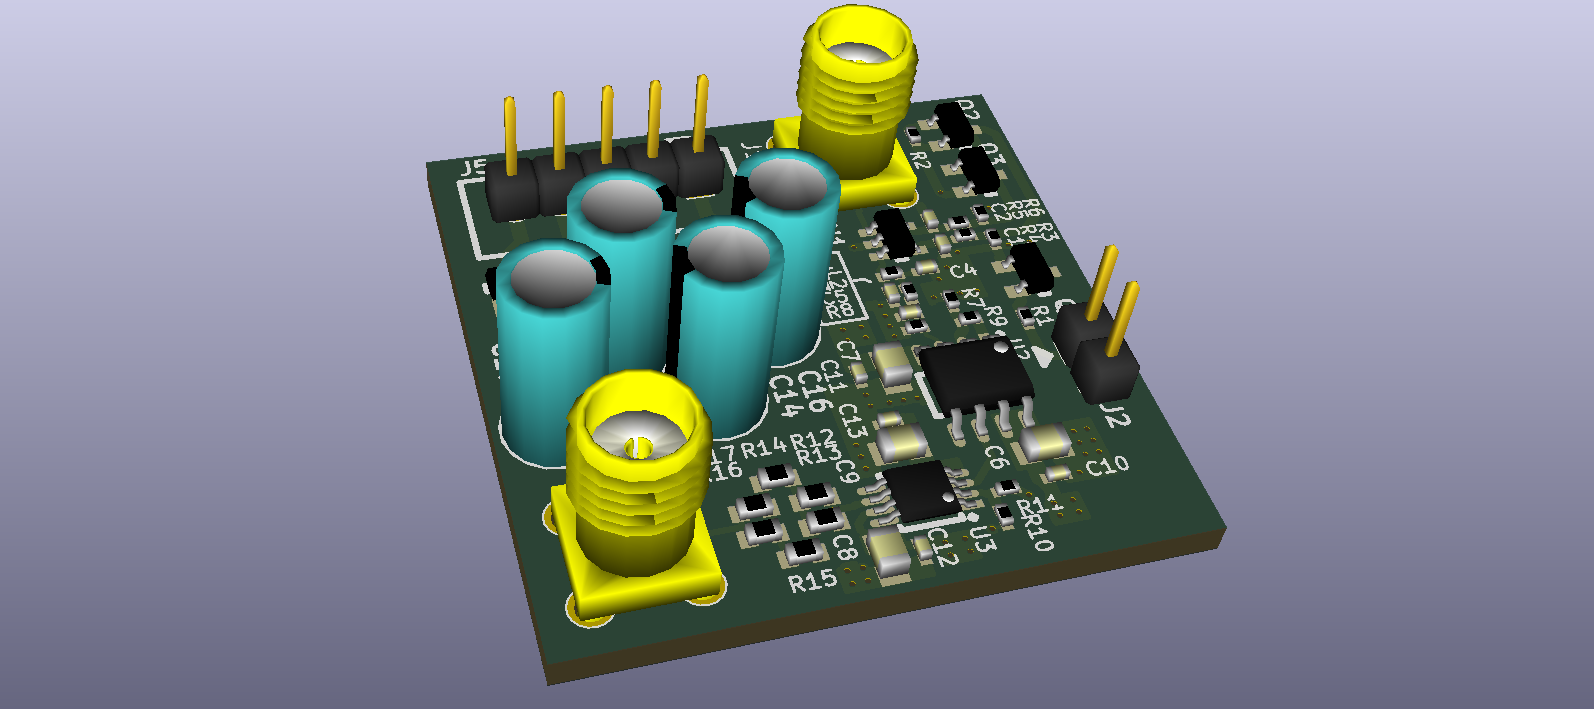
\includegraphics[width=4in]{outamp3d.png}
\caption{Output Amplifier PCB, 3D render}
\label{fig:outamp3d}
\end{figure}

The output amplifier must take small signals, at $–8.5\;\mr{dBm}$ as they arrive from
the synthesizer, and output the full $15\;\mr{dBm}$  signal. For design margin, a $16.5\;\mr dBm$
 output amplitude is assumed. This gives a required gain of $25\;\mr dB$. An
additional $6\;\mr dB$ gain is required to compensate for the insertion loss of the
termination, giving a total required gain of $31\;\mr dB$.  A gain of $31\;\mr dB$ from $1\;\mr kHz$
(practically DC) to $150\;\mr MHz$ is difficult to achieve, particularly with the very
large absolute amplitude of $21\;\mr dBm$ at the output. We chose to use two gain
stages of $15.5\;\mr dB$ each. The final stage is a THS3001 operational amplifier, as
it supports the high slew rate, high voltage and high output current required.
This is a very expensive amplifier, though, so we used the AD8000 (similar
specifications, but with a lower maximum supply voltage) for the first stage.
The synthesizer allows amplitude control, but this control is applied at the
digital stage, resulting in a loss of DAC resolution. To get more range at full
resolution, we included a MAADSS0008 switchable $15\;\mr dB$ attenuator in the output
amplifier's signal path.

\subsection{Microprocessor}
For our system's microprocessor, we used the Atmel SAM4S16C ARM Cortex-M4
microcontroller. In the final product, we will switch to a less expensive
microcontroller in the SAM4S line with a smaller amount of memory, after we
have determined the amount needed.

In the current prototype, we are using the Atmel SAM4S Xplained evaluation kit;
the final product will use the chip by itself.

\section{Use}
The purpose of this device is provide students with tangible data when analyzing
circuits. As shown in \autoref{fig:contextdiag}, the device is to be connected between
a PC and a device under test; the user can initiate an analysis using the supplied software.
